\chapter{Implementation Details}
\label{Chapter4}
In this chapter, a bottom-up approach will be followed in order to present all the parts that make up the challenge itself:
\begin{itemize}
\item \textbf{Logic design}, the Block Cipher at Register Transfer Level, including all its internal components and subparts
\item \textbf{Bistream}, the files coming from an HDL wrapper needed to configure the FPGA
\item \textbf{Middleware}, the library used to link the design to the MCU on the embedded platform (i.e. \emph{Overlay})
\item \textbf{Web server}, the framework used to build and host the web server directly on the board (i.e. \emph{CherryPy})
\item \textbf{Front-end}, the web page displaying the GUI to the end-user.
\end{itemize}
\section{Logic design}
The lowest layer of the whole project consists of a vulnerable Block Cipher, implemented with a parallelism of 256 bits.
This architecture is capable of taking a unique seed (\emph{exactly} 256-bits long) together with a plaintext of variable size (\emph{at least} 256-bits long) in order to generate the corresponding ciphertext, whose length will be determined by the latter input.
Such process is based on two main PRNGs, and the operation should theoreticall be non-invertible: the vulnerability consists in eliminating the non-linearity that defines this very same property.

Note that all the source VHDL files describing the following components were commented extensively, and can be found in the ``VHDL/VHDL.srcs/sources\_1/new/'' directory.
\subsection{LFSR}
A Linear Feedback Shift Register is represented by a set of D Flip-Flops linked in succession, where the output of each represents the input of the following one: the primary intake of this structure is represented by the D port of the first FF, whereas the Q pin of the last one serves as the main product.
Such arrangement acts as the dividend of the operation that is being implemented: in fact, this kind of block performs nothing more than a division between polynomials.

The divisor is instead made up by a set of intermediate bits (that will be called ``taps'') which all go through an XOR port in order to generate a feedback signal that ends up in the first element of the chain.
Their position can vary, but there exists only one combination of them that makes the related polynomial primitive.
This definition refers to the fact that, during its activity, a LFSR is capable of transitioning amongst a limited amount of states.
When its divisor is a primitive polynomial, then it will be referred to as a \textbf{maximal-length} LFSR, meaning that it's able to cycle over all the 2\textsuperscript{N}-1 possible states (where N is the number of bits, i.e. 256 in this context).

Its computation is pseudo-random, as it always has to start from an initial value (called ``seed'') different from zero, and the sequence of phases it will trantition into will always be the same (depending on the hardwired taps it includes).
In this case, the LFSR starts exactly in this \emph{absorbing} state, being stuck with all its bits at 0, until the user begins to load the message that will need to be encoded.

As the vulnerability had to be well-hidden inside the design in question, this block needed to be heavily modified in order to include an additional internal entity, referred to as \emph{scrambler} inside the code.
The purpose of the latter is to provide the same sequential functionality of the ALFSR (see below), coupled with a convoluting process aimed at making its real purpose more obscure to the contestant.
\begin{figure}[!ht]
\vspace{0.5cm}
\includegraphics[width=\textwidth]{images/lfsr_partial.png}
\caption{Noteworthy portion of the LFSR.}
\end{figure}
\subsection{ALFSR}
This device is essentially the same as the one described above, with the only difference that its seed is loaded parallelly only once, and then the register is left running virtually forever with no other user input.
This is the actual reason for which this structure is given the attribute \textbf{autonomous}, as in Autonomous Linear Feedback Shift Register (ALFSR).
It represents the second main contribution to the encoded product of the Block Cipher, and its output signal is still serial.
\begin{figure}[!ht]
\vspace{0.5cm}
\includegraphics[width=\textwidth]{images/alfsr.png}
\caption{Schematic of the ALFSR.}
\end{figure}
\subsection{FA}
This is a simple fulladder with carry in and carry out support (implemented by means of a simple D Flip-Flop). It is characterized by the following equations:
\begin{equation}
S=A\oplus B\oplus C_{in}
\end{equation}
\begin{equation}
C_{out}=(A\cdot B)+(A\cdot C_{in})+(B\cdot C_{in})
\end{equation}
where A represents the output of the combinational network (detailed later), or in principle the contribution of the LFSR, while B is the output of the ALFSR.
\begin{figure}[!ht]
\vspace{0.5cm}
\includegraphics[width=\textwidth]{images/fulladder.png}
\caption{Schematic of the fulladder.}
\end{figure}
\subsection{EDGE}
This circuit represents an enabler for the vulnerability: as soon as its main output is asserted, the whole Block Cipher gets trivially reduced to the LFSR only.
The two key points are: how the purposefully-injected fault is triggered, and in which way the extreme simplification of the top level design is achieved.

Starting from the first matter, this architecture was implemented by means of a peculiar Mealy State Machine which closely monitors the feedback signal of the LFSR during its initialization.
If such bit goes to 1 exactly once every four clock cycles (strictly: 0001, 0001, 0001, ...), then, whenever the LFSR acknowledges the validity of its output, the special internal enable is activated.
Note that the final value for its principal output signal gets sampled on a rising edge of the valid bit: this was the main reason for which this structure was called ``EDGE''.
Instead, as soon as even a single feedback does not respect the above sequence, the product of this block gets irreversibly stuck at 0 (or until the next reset, at least).

On the other hand, the vulnerability itself is achieved in conjunction with the aforementioned \emph{scrambler} and the combinational network, in such a way that the contribution of the ALFSR simply gets omitted from the final operation. More details will follow.
\begin{figure}[!ht]
\vspace{0.5cm}
\includegraphics[width=\textwidth]{images/enabler.png}
\caption{Schematic of the enabler.}
\end{figure}
\subsection{NET}
This combinational network represents the last element that makes up the vulnerability of the design in question. It has three main functionalities:
\begin{enumerate}
\item completing the ``secondary ALFSR'' located inside the real LFSR by creating the feedback network for the so-called \emph{scrambler}
\item computing the sum between the outputs of the LFSR and of the ALFSR$'$, with support for the carry bit as well
\item estimating the carry out of the previous arithmetic operation.
\end{enumerate}

This organization of logic gates is aimed at recreating the same output of the main ALFSR in order to put it in XOR with the product of the LFSR, effectively anticipating the contribution of the subsequent fulladder.
The hardcoded equation for the bit that will represent the first operand of the main sum in the top level structure is:
\begin{equation}
NET_{out}=LFSR_{out}\oplus \left((ALFSR'_{out}\oplus C'_{in})\cdot EDGE_{out}\right)
\end{equation}
where the output of ALFSR$'$ and the carry in are identical to the ``real'' ones, but are computed in a much more cryptic and concealed way (the taps of the scrambler are the same as the ones found in the primary ALFSR, which in turn features a different divisor from the one hardcoded in the LFSR---however, all these registers are maximal-length).

Note that this whole functionality is gated by the output bit of the enabler: if the latter remains at 0, then the output of this network will be equal to the contribution of the LFSR only, and the user won't notice any defect in the response.
\begin{figure}[!ht]
\vspace{0.5cm}
\includegraphics[width=\textwidth]{images/combinational_network.png}
\caption{Schematic of the combinational network.}
\end{figure}
\subsection{BlockCipher}
The top level entity is thus made of the two main contributions of the LFSR and the ALFSR, the outputs of which are added one by one after going through the application-specific additional logic.
The ciphertext is marked as ``valid'' only after both registers are loaded correctly: this information is conveyed by means of a dedicated output bit as well.

Looking at it from this level, the vulnerability can be attributed to an additional ALFSR, here called ALFSR$'$, which is disassembled and spread across the whole design: the register part (\emph{scrambler}) is inside the LFSR, while the XOR for feedback creation is inside the combinational network.
On the other hand, also the fulladder is regenerated again within the ``NET'', in such a way that the actual output of the primary fulladder will be represented by:
\begin{equation}
FA_{out}=LFSR_{out}+ALFSR_{out}-(ALFSR'_{out}\cdot EDGE_{out}),\quad ALFSR_{out}=ALFSR'_{out}
\end{equation}
which represents the final outcome of the encryption process.

Note that all the debug signals required by the challenge and both the principal products (ciphertext and valid bit) are rendered sequential by means of output D Flip-Flops, in order to make the interface with the subsequent layers possible.

Lastly, this implementation was tested by means of an appropriate testbench, located inside the ``VHDL/VHDL.srcs/sim\_1/new/'' directory together with many useful input memory files.
Any simulation of ``tb\_BlockCipher.vhd'' would lead to the creation of several output files in as well (placed in ``VHDL/VHDL.sim/sim\_1/behav/xsim/''): they include the collection of values that each signal shown on the final webpage takes on during the whole runtime, in order to handily compare them and check their correctness.
\begin{figure}[!ht]
\vspace{0.5cm}
\includegraphics[width=\textwidth]{images/top_level.png}
\caption{Entire schematic of the Block Cipher, showing the internal connections between all its fundamental components.}
\end{figure}
\section{Bitstream}
\label{bitstream}
The design described above had to be converted into a custom IP, which was in turn included within an HDL wrapper in order to go through the necessary steps of implementing its logic functionalities onto the embedded board.
A detailed documentation aimed at this goal was kindly provided by \textbf{Coralie Allioux}, who created the \emph{Tutorial Vivado 2020.2.pdf} file expressely for this reason.

The Vivado project used alongside that paper is located in the ``BlockCipher/project\_1/'' directory, while ``BlockCipher/ip\_repo/'' was automatically created and contains the required file structure for the aforementioned IP.
For the sake of convenience, the input netlists of the bitstream generation process are duplicated inside ``PYNQ/Board\_Files/src/'', whereas ``PYNQ/Board\_Files/gen/'' contains the resulting files needed to configure the FPGA on the remote platform (\textbf{.bit}, \textbf{.hwh} and \textbf{.tcl}).
Please note that these three MUST have the same name in order to properly work with \emph{Overlay}, so a refactoring will likely be needed before sending them to the PYNQ.

All the signals that make up the I/O list of the Block Cipher had to be instantiated as 32-bit registers inside the AXI4 peripheral because of a software limitation of Vivado: this way, the parallel in going into the ALFSR (originally 256-bits long) had to be split into 8 different registers that would later get concatenated internally.
A table containing the current addressing offsets of such registers is here provided: those are the memory locations that higher-level layers will need to access when trying to interact with the logic design.
\begin{table}
\centering
\begin{tabular}{| l | c |}
        \hline
        \textbf{Name} & \textbf{Offset}\\ \hline
        \hline
        ALFSR\_PARALLEL\_IN7 & 0x00\\ \hline
        ALFSR\_PARALLEL\_IN6 & 0x04\\ \hline
        ALFSR\_PARALLEL\_IN5 & 0x08\\ \hline
        ALFSR\_PARALLEL\_IN4 & 0x0C\\ \hline
        ALFSR\_PARALLEL\_IN3 & 0x10\\ \hline
        ALFSR\_PARALLEL\_IN2 & 0x14\\ \hline
        ALFSR\_PARALLEL\_IN1 & 0x18\\ \hline
        ALFSR\_PARALLEL\_IN0 & 0x1C\\ \hline
        LFSR\_SERIAL\_IN & 0x20\\ \hline
        SEQUENTIAL\_ENABLE & 0x24\\ \hline
        CLOCK & 0x28\\ \hline
        RESET & 0x2C\\ \hline
        LOAD\_0 & 0x30\\ \hline
        LOAD\_A & 0x34\\ \hline
        LFSR\_DEBUG\_OUT & 0x38\\ \hline
        ALFSR\_DEBUG\_OUT & 0x3C\\ \hline
        FA\_DEBUG\_OUT & 0x40\\ \hline
        EDGE\_DEBUG\_OUT & 0x44\\ \hline
        NET\_DEBUG\_OUT & 0x48\\ \hline
        RESULTS\_SERIAL\_OUT & 0x4C\\ \hline
        VALID\_DATA & 0x50\\ \hline
\end{tabular}
\caption{AXI4 peripheral registers addressing.}
\end{table}
\section{Middleware}
PYNQ is an open-source project made by Xilinx\textsuperscript{\tiny{\textregistered}} to better take advantage of the functionalities included in the embedded microcontroller.
Using Python libraries, designers can exploit the benefits of programmable logic and microprocessors to build more capable electronic systems.

The related SoC is based on a dual-core ARM\textsuperscript{\tiny{\textregistered}} Cortex\textsuperscript{\tiny{\textregistered}}-A9 processor (referred to as the Processing System or PS), integrated with FPGA fabric (the Programmable Logic or PL).
The PS subsystem includes a number of dedicated peripherals (memory controllers, USB, UART, I\textsuperscript{2}C, SPI, etc.) and can be extended with additional hardware IP in a PL architecture.

Overlays, or hardware libraries, are to be intended as an interface between the Processing System and the FPGA. This way, they can be used to accelerate a software application or, in general, to integrate it with a hardware layer.
In this context, \emph{Overlay} is used to transform the Block Cipher into a Python script.
\begin{figure}[!ht]
\vspace{0.5cm}
\centering
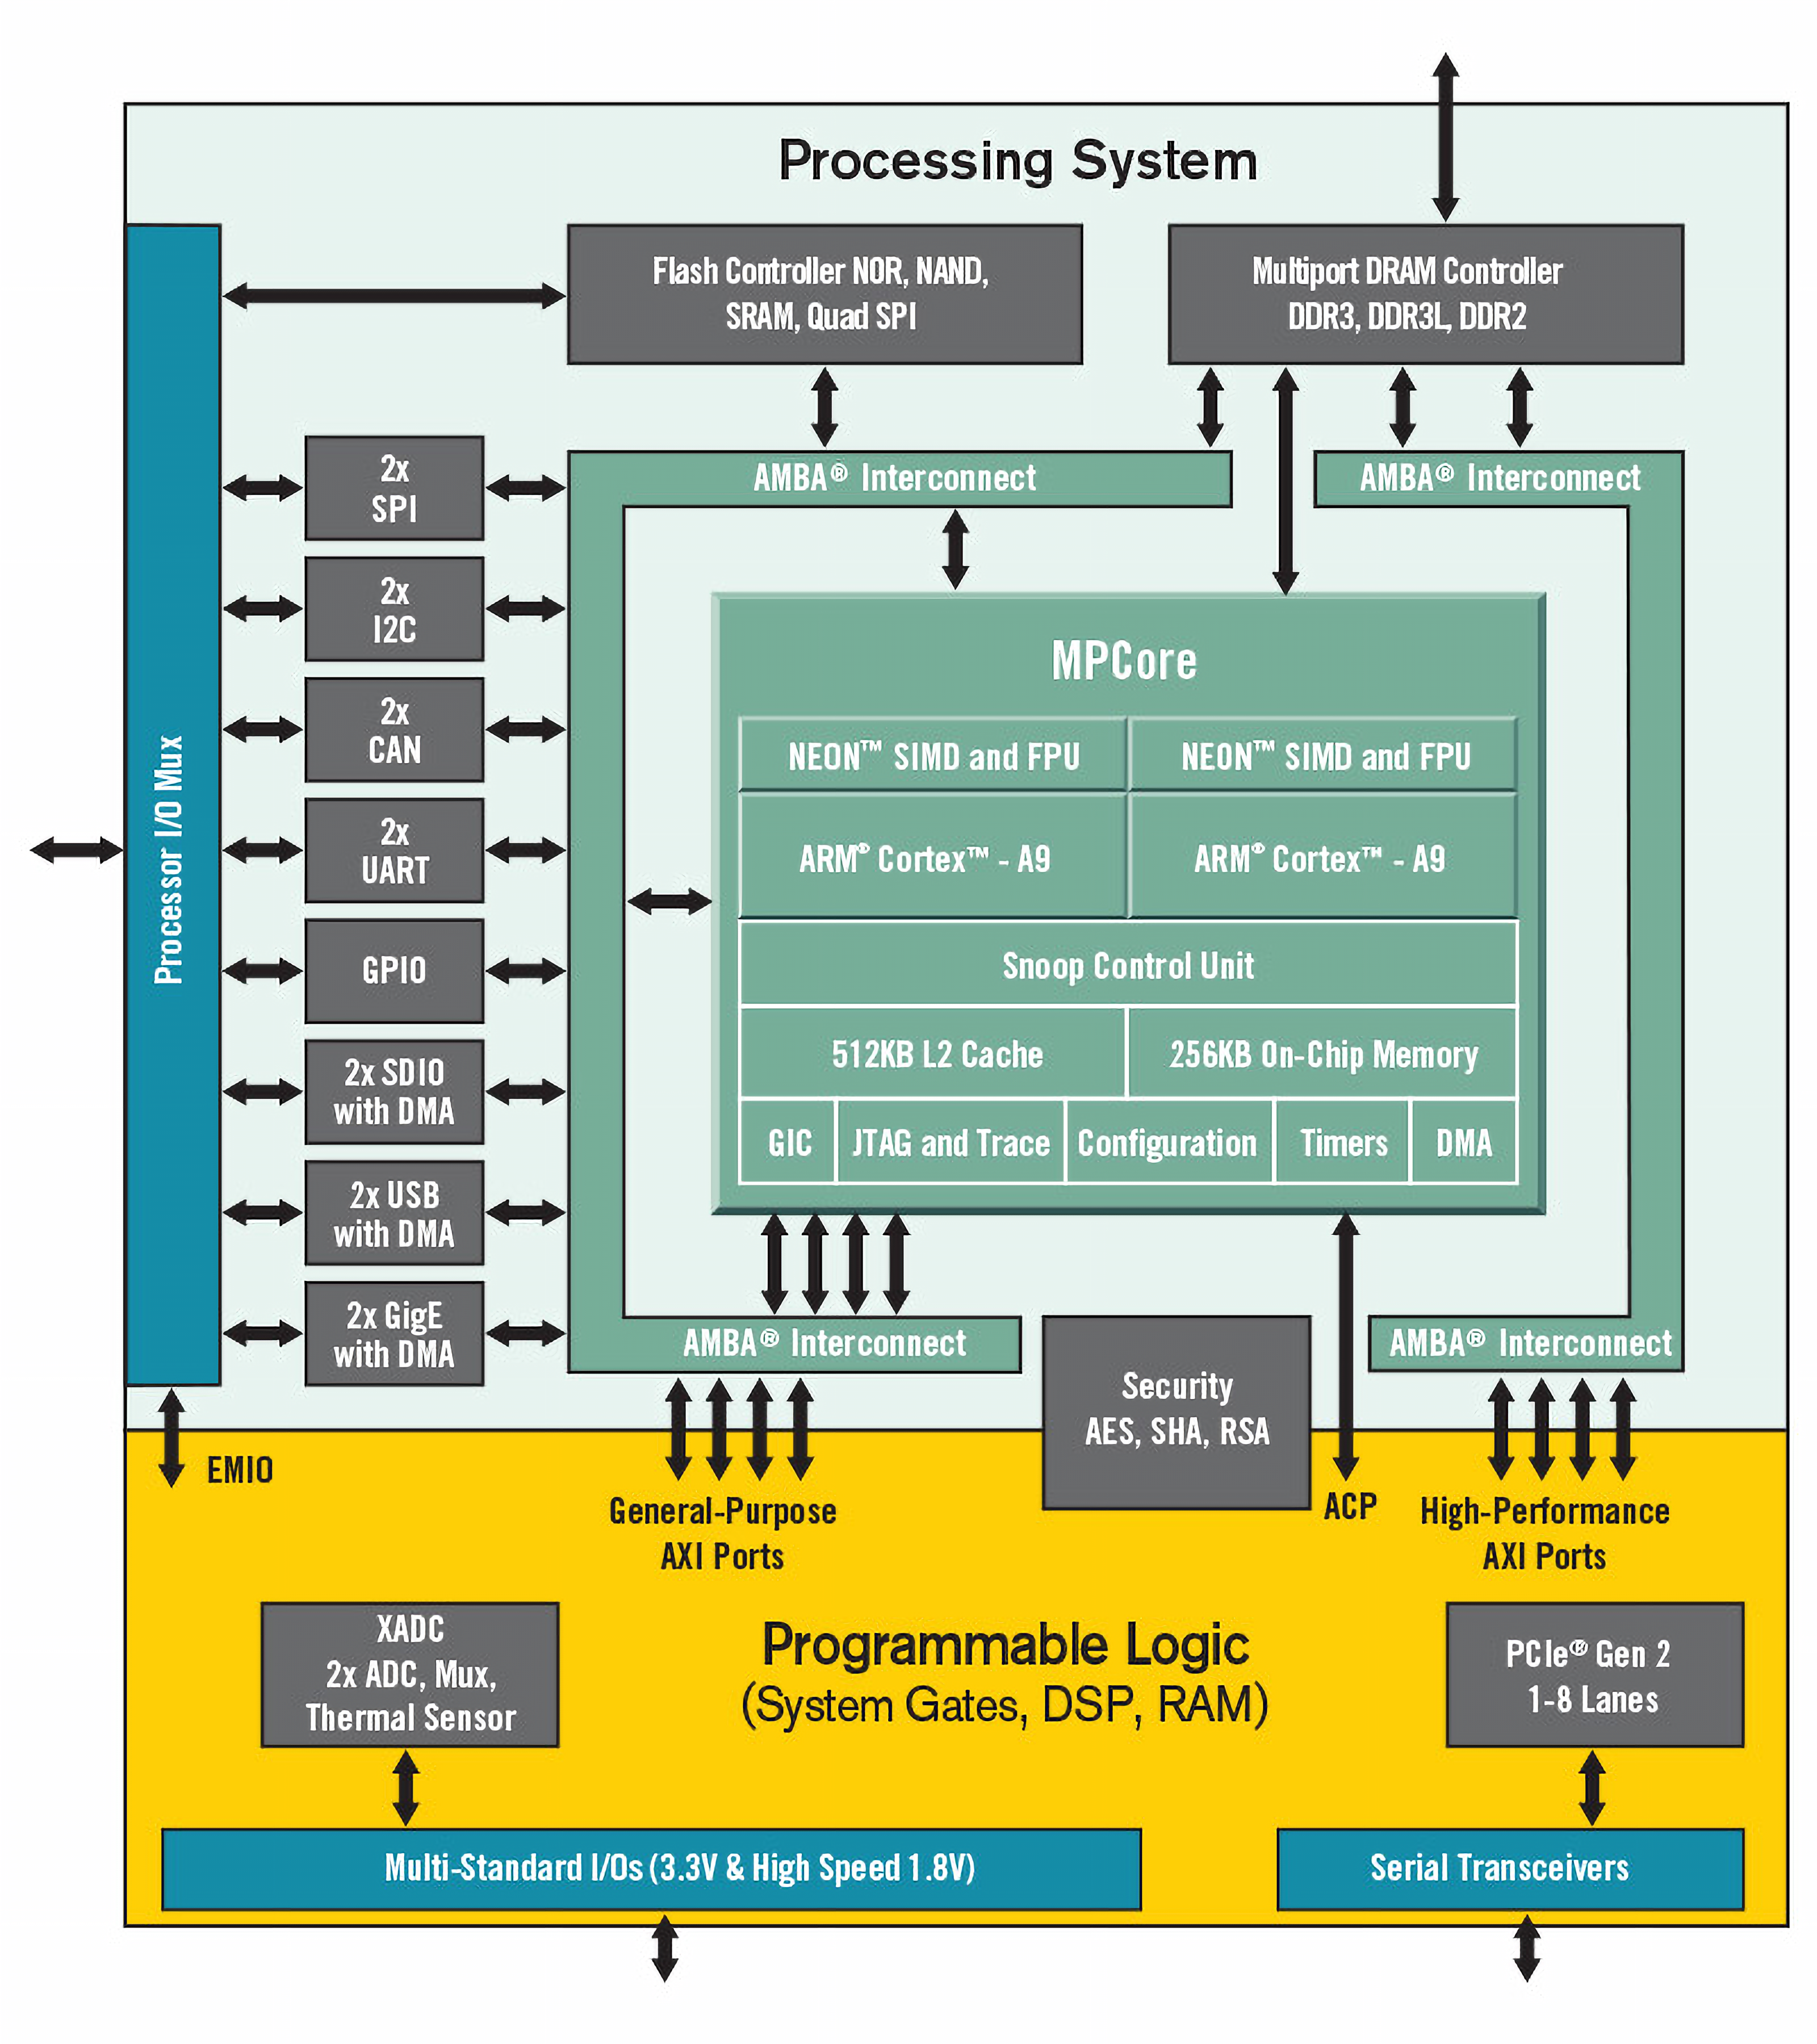
\includegraphics[width=0.75\textwidth]{images/zynq.png}
\caption{Schematic of a Zynq SoC.}
\end{figure}
\subsection{Board interfaces}
The Zynq has 9 AXI registers used to interface between the PS and the PL. On the PL side, there are 4 AXI Master HP (High Performance) ports, 2 AXI GP (General Purpose) ports, 2 AXI Slave GP ports and 1 AXI Master ACP port.
Python code running on PYNQ can access the IP connected to an AXI Slave, which in turn is linked to a GP port (MMIO is used to achieve this association).

Any IP connected to the AXI Slave GP port will be mapped into the system memory map: MMIO can be used access all mapped locations, in such a way that any read/write command is a single transaction to transfer 32 bits of data from/to a memory section.
The \textbf{.hwh} file is responsible, among other functionalities, of storing the memory map of the selected architecture: inside the <MODULES> section, the <ADDRESSBLOCKS> tag specifies the offset associated to each port of the design.

Note that all registers have a fixed size (e.g. 32-bits), hence, whenever a single bit has to be managed by means of the \emph{std\_logic} VHDL type, it will be sufficient to bind the corresponding signal to just one bit of it (the LSB in this case).
\subsection{Driver}
Starting from the outcomes of the bitstream generation process, the \textbf{.bit} file is loaded inside the PL, while the \textbf{.hwh} is used for the interface with the PS.
Once an overlay has been instantiated, it is linked to the driver that actually calls the read/write instruction, making the commun ication with the IP possible.

The \textbf{CipherDriver} (cfr. ``PYNQ/UserInterface/CypherDriver.py'') is a class used to expose a method that performs the communication to the PL.
Starting from the input values of the Block Cipher sent by the GUI (more on that later), it returns a JSON containing the relevant outputs of the same design.
\section{Web server}
The previous services were then made accessible from remote by means of a web server running on the PS side of the board.
Such back-end is based on the \emph{CherryPy} Python web framework, which links local resources to a public URL.

Inside the \emph{web\_server.py} file (placed in ``PYNQ/UserInterface/'') the application is launched and is capable of managing HTTP requests coming from an external host.
This function is then linked to the IP address of the network interface of the board itself, with a specified port (where 8080 is the default).
Then, whenever a POST is requested from the client, the server responds by means of a GET that delivers the \emph{webpage.html} file (located in the same folder), containing the dynamic data that the custom IP itself will have returned.
\section{Front-end}
The Graphical User Interface was here implemented by means of a webpage accessible through any popular browser. This solution is thought to be the best choice considering the ease of use, availability of functionalities and general accessibility.

The GUI is made up of four different parts:
\begin{itemize}
\item static HTML webpage
\item CSS-based interactive elements
\item several JS scripts
\item CTF challenge source code and previews.
\end{itemize}
\subsection{Static HTML}
Right after connecting to the provided URL, the contestant is presented with a straightforward webpage which contains four main sections:
\begin{itemize}
\item the challenge background, which gives the player some basic information regarding its scope, while setting the mood of the game thanks to a short backstory
\item a table containing the list of components that make up the implemented logic, together with the links to download and/or preview the source code
\item the input form containing two fields to be filled by the participant---above this segment, a brief paragraph gives the user some additional information regarding the accepted formats of the input data
\item many output labels that will populate with the response coming from the PYNQ, including both the main output signals of the Block Cipher and a few other relevant signals that are deemed very important for debugging purposes.
\end{itemize}

The HTML heavily relies on \emph{Bootstrap}, a popular front-end library widely used in web development that greatly simplifies the formatting and adaptability of the webpage.
\begin{figure}[!ht]
\vspace{0.5cm}
\includegraphics[width=\textwidth]{images/home.png}
\caption{Homescreen of the challenge, zoomed out in order to display all the described elements.}
\end{figure}
\subsection{JavaScript snippets}
The JavaScript code implements many functionalities that would otherwise not be possible by HTML alone:
\begin{itemize}
\item all input and output fields are resized automatically depending on their content---this greatly improves readability and makes the flow of the challenge much smoother
\item the preview system of the VHDL netlists is implemented through JS
\item the `Clear' button resets the whole input form for convenience
\item the actual communication between the front-end GUI and the back-end hosted on the PYNQ is carried out thanks to Ajax POST requests; more specifically:
        \begin{enumerate}
        \item the used fills the input data and presses the `Send' button
        \item the input data is used to generate a POST request that is delivered to the back-end server
        \item the back-end, after elaborating the data and collecting the output from the FPGA, responds to the Ajax request with a string to be parsed into a dictionary
        \item a JS script collects the incoming object and uses its content to populate the output fields of the HTML, without the need to reload the webpage.
        \end{enumerate}
\item both input text fields are checked locally in real time (rather than on the \emph{CherryPy} server) to make sure the data being written is well formatted and doesn't contain invalid messages---the user is not able to send the information unless all parsing constraints are satisfied.
\end{itemize}
Regarding the last point, it's important to notice that there exist a couple of edge cases that need to be taken into consideration: if any of the three PRNGs (LFSR, ALFSR and ALFSR$'$) never leaves the ``absorbing'' state, it remains forever stuck and the acknowledge signal will not display the required rising transition.
As the middleware of this application waits for that particular edge of the valid flag in order to return the correct values, it is in fact crucial to avoid this type of situation in order not to end up inside an infinite loop.
Therefore, both the seed and the plaintext must not be made of all zeros; additionally, the former cannot be formed by all ones either, due the related \emph{scrambler} getting loaded with the complemented version of such value (i.e. all zeros, again).

The ``PYNQ/UserInterface/webpage.html'' file contains, among many other pieces of code, the snippets dedicated to this kind of checking:
if any of the input fields passes the initial length test, but would lead to the previously mentioned infinite loop, the request is not even forwarded to the board at all, while every output label gets abruptly overwritten with the message \textcolor{red}{\textbf{PROCESS TIMEOUT}} to alert the user.
\begin{figure}[!ht]
\vspace{0.5cm}
\includegraphics[width=\textwidth]{images/parsing.png}
\caption{Example of failed parsing rules in the input form: the `Send' button is disabled.}
\end{figure}
\begin{figure}[!ht]
\vspace{0.5cm}
\includegraphics[width=\textwidth]{images/success.png}
\caption{Successful request + response (including contest victory).}
\end{figure}
\subsection{Preview system}
A key part of the challenge is the ability for the user to access the source code to try and reverse engineer it, possibly finding the correct solution.
As explained in the previous section, the webpage contains a list of links to download the source files and to preview them directly online.

Each of the preview buttons launches a pop-up (more specifically a \emph{modal window}) which captures the source code of the chosen source file.
The latter is already well formatted and color-coded inside the corresponding external HTML file, having been generated by means of the contents of ``PYNQ/Previews/'' in the following way:
\begin{enumerate}
\item cut-paste the desired VHDL netlist inside \emph{test.html}
\item open the latter inside any browser---the \emph{run\_prettify.js} script will be launched automatically (all credits go to \textbf{Google Inc.})
\item save the newly visualized webpage as a \textbf{.html} file with an arbitrary name, and move it to ``PYNQ/UserInterface/previews/''.
\end{enumerate}
This way the VHDL source code is visible on the fly, without the need to download it on a local machine to be opened with a suitable text editor/IDE.
\begin{figure}[!ht]
\vspace{0.5cm}
\includegraphics[width=\textwidth]{images/net.png}
\caption{Preview page of the combinational network.}
\end{figure}